\section{The Gaussian chain: diffusion breaks locality}
\label{sec:gaussian}

\begin{figure*}[t]
  \centering
  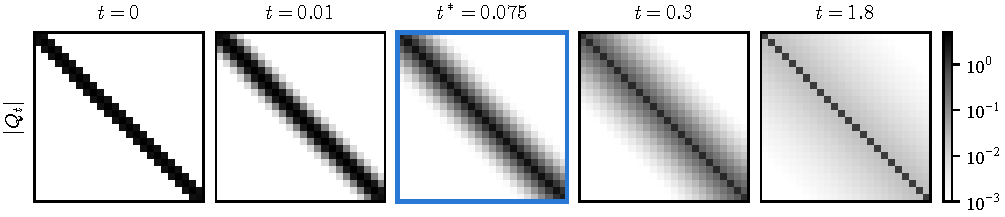
\includegraphics{fig_locality}
  \caption{Noise makes the score non-local. Magnitude of the matrix $\mathbf Q_t$ in the score
  $\mathbf S_t(\mathbf x)=-\mathbf Q_t\mathbf x$ of the Gaussian chain ($\alpha=0.85$, $L=24$) at five noise levels, on
  a log colour scale. At $t=0$ it is tridiagonal; at large $t$ it tends to the identity; in between, at
  $t^{*}\simeq0.075$ (framed), it is furthest from tridiagonal.}
  \label{fig:locality}
  % src: closed form, tools/paper_figs/make_paper_figures.py::fig_locality (t* = 0.0753 printed by the generator)
\end{figure*}

As an exactly solvable baseline, consider the stationary Gaussian chain
\begin{equation}
    a_{k+1}=\alpha a_k+\eta_k,
    \qquad \eta_k\sim\mathcal N(0,1-\alpha^2),
\end{equation}
where $\alpha\in(-1,1)$ sets the correlation between consecutive sites and the noise variance $1-\alpha^2$ keeps the
chain stationary with unit variance. Its joint distribution is Gaussian,
$p_0(\mathbf a)=\mathcal N(\mathbf 0,\boldsymbol\Sigma_0)$ with $(\boldsymbol\Sigma_0)_{ij}=\alpha^{|i-j|}$, and its
precision matrix $\mathbf Q_0=\boldsymbol\Sigma_0^{-1}$ is tridiagonal: this is the Markov property, written as a
statement about the score.

Under the noise of \cref{eq:ou_corruption} the data stay Gaussian,
\begin{equation}
    p_t(\mathbf x)=\mathcal N(\mathbf 0,\boldsymbol\Sigma_t),
    \qquad
    \boldsymbol\Sigma_t
    =e^{-2t}\boldsymbol\Sigma_0+\Delta_t\mathbf I,
\end{equation}
so the score is exactly linear:
\begin{equation}
    \mathbf S_t(\mathbf x)
    =-\mathbf Q_t\mathbf x,
    \qquad \mathbf Q_t=\boldsymbol\Sigma_t^{-1}.
\end{equation}
While $\mathbf Q_0$ is tridiagonal, $\mathbf Q_t$ is dense for $t>0$ (\cref{fig:locality}). Diffusion turns a locally
structured chain into a distribution whose score is not local, even though the distribution stays Gaussian. The effect
is strongest at an intermediate noise level, $t^{*}\simeq0.075$ for $\alpha=0.85$, and fades at large $t$, where the
noise dominates.
% src: t* = 0.0753, fig_locality / fig_locality_curve

So locality cannot simply be imposed on the denoiser. A denoiser that only looks at the two neighbours of each site
has a relative score error of $0.20$ even with unlimited data. The structure survives elsewhere: the posterior
$p_t(\mathbf a\mid\mathbf x)$ of \cref{eq:posterior_chain} is still a chain, because the noise adds one factor per site
and no new link. For the Gaussian chain, inference along this chain returns $-\mathbf Q_t\mathbf x$ exactly in $O(L)$
operations, without ever forming $\mathbf Q_t$. The next sections do the same for any kernel.
% src: thesis tools/fig_ch10.py::windowed_oracle([1]) = 0.2023 (alpha=0.85, L=32, twelve levels)
